% !TEX root = ../my-thesis.tex
%
\selectlanguage{english}  
\chapter{\textcolor{ctcolormain}{Colonization pattern of \Qp in Mediterranean mountains abandoned croplands: a study case from Sierra Nevada (Spain)}}\label{sec:coloniza}




\mbox{}
\vfill
{\color{ctcolormain}\textbf{Antonio J. Pérez-Luque}}; Francisco J. Bonet-García \& Regino Zamora (In prep.)


\newpage

\paragraph{Abstract} \mbox{} \\
Land abandonment is a major global change driver in the Mediterranean region where anthropic activity has played an important role shaping landscape configuration. Understanding the woodland expansion towards marginal areas (abandoned crops) is critical to develop effective management strategies. In this work we analyze the colonization pattern of abandoned croplands by \emph{Quercus pyrenaica} in Sierra Nevada. We aimed to assess differences among populations in the rear edge of its distribution. For this purpose we characterized \emph{(i)} the colonization pattern of \emph{Q. pyrenaica}, \emph{(ii)} the structure of the seed source (mature forest), and \emph{(iii)} the abundance of the main seed disperser (European jay, \emph{Garrulus glandarius}). The study was conducted in five abandoned croplands located in two representative populations of \emph{Q. pyrenaica} located in contrasting slopes. We sampled three habitat types: mature forest, edge-forest and abandoned cropland. A total of 83 plots (10 x 30 m) were sampled. In each plot all tree individuals were counted. Basal diameter and height of each tree specimen were measured and sapling abundance was calculated. Abundance of European jay was determined by bird census (7-year) (line-transect method). Sapling abundance was different between northern and southern \emph{Q. pyrenaica} populations. However, no differences on sapling abundance were observed among habitat types. Abundance of jay does not differ significantly between sites. On the other hand, forest structure showed differences between populations. Differences in colonization pattern could be explained by different management histories and (different land-use intensities) before abandonment of the croplands (biological legacies) and cattle management. 
practices.

\newpage

\section{Introduction}\label{sec:coloniza:intro}

Land-use change is considered the main global change driver worldwide \autocites{Butchartetal2010GlobalBiodiversity,Winkleretal2021GlobalLand} affecting biodiversity \autocites{Sala2000GlobalBiodiversity}, modifying ecological processes \autocites{Lindenmayeretal2012LandUse}, and altering the provision of ecosystem services \autocites{Hasanetal2020ImpactLand}. Land-use change varies geographically, being the croplands abandonment and afforestation the main processes in the Northern hemisphere \autocites{Winkleretal2021GlobalLand,ReyBenayas2007AbandonmentAgricultural}. In Mediterranean region, where anthropic activity has played an important role shaping landscape configuration, cropland abandonment has been widespread during the second half of the last century \autocites{Piasetal2014ColonizationAbandoned,ValbuenaCarabanaetal2010HistoricalRecent}, and land-use change models predict an increase in this trend in the future \autocites{Rounsevelletal2006CoherentSet,PerpinaCastilloetal2021ModellingAgricultural}. The abandonment of traditional activities has left many Mediterranean landscapes in an almost barren state, with poor vegetation cover \autocites{Sheffer2012ReviewDevelopment, ReyBenayas2007AbandonmentAgricultural}. Consequently, a natural vegetation regeneration process started with a spontaneously recovery of abandoned croplands \autocites{Debusscheetal1999MediterraneanLandscape,PenuelasBoada2003GlobalChangeinduced,AlvarezMartinezetal2014InfluenceLand,Nataleetal2007StudyTree,Piussi2000ExpansionEuropean}. 

\Qpy woodlands, like other forest formations in the Mediterranean region, have been subjected to intense anthropogenic pressures over time \autocites{GarciaJimenez20099230Robledales, AlbaSanchezetal2021EarlyAnthropogenic}, which have led to the reduction of their distribution area, as well as to the modification of their floristic and structural patterns \autocites{Gavilanetal2000EffectsDisturbance,Calvoetal1999PostfireSuccession,Tarregaetal2006ForestStructure}. Historically, the woodlands of \Qp have been exploited mainly for firewood, charcoal and tannins \autocites{RuizdelaTorre2006FloraMayor,SanchezPalomaresetal2008EstacionesEcologicas}. Some areas were also burned and thinned to create pastures with low densities of mature trees that provide acorns, firewood and large areas for grazing \autocites{HerreraCalvo2016UsoPastoral,Alvarezetal2009CambiosEstructura,ValbuenaCarabanaGil2017CentenaryCoppicing}. All these anthropogenic processes have transformed the oak woodlands in a deep way that it is difficult to find stands that can be considered natural forests \autocites{RuizdelaTorre2006FloraMayor}. 

However, the abandonment of traditional uses since the middle of the last century \autocites{MacDonaldetal2000AgriculturalAbandonment}, has caused a decrease in anthropogenic pressure on Mediterranean forest ecosystems \autocites{ValbuenaCarabanaetal2010HistoricalRecent}, being particularly important for mountain areas \autocites{Nataleetal2007StudyTree, AlvarezMartinezetal2014InfluenceLand,JimenezOlivenciaetal2015MedioSiglo,JimenezOlivenciaetal2015EvolucionUsos,Piasetal2014ColonizationAbandoned}. The dramatic rural exodus occurred in mountain areas due to changes in socio-economic conditions \autocites{EuropeanEnvironmentAgency2010EuropeEcological}, provoked an abandoned of traditional activities and significant environmental changes \autocites{MacDonaldetal2000AgriculturalAbandonment, Nataleetal2007StudyTree, AlvarezMartinezetal2014InfluenceLand,Piussi2000ExpansionEuropean,Rutherfordetal2008AssessingLanduse,Zimmermannetal2010EffectsLanduse}. This decrease in anthropogenic pressure has paradoxically provoked that many of the \Qp oak stands present a state of advanced degradation, showing growth stagnation, lack of fruiting, and also sings of branch dieback  \autocites{Canellasetal2004GrowthResponse, Bravoetal2008SelviculturaMontes, ValbuenaCarabanaGil2014EfectosGestion, PiqueVericat2015EvolutionPerspectives, Piqueetal2018Spain}. 

Moreover the abandonment of mountain agricultural areas is causing an increase in forest expansion via the spontaneously recovery of vegetation \autocites{Piussi2000ExpansionEuropean}, that can causes a homogenization of the landscape \autocites{Mietkiewiczetal2017LongtermChange} and a loss of biodiversity \autocites{Zimmermannetal2010EffectsLanduse}. Therefore, understanding the woodland expansion towards marginal areas (abandoned crops) is critical to develop effective management strategies. 

In this work we analyze the colonization pattern of abandoned croplands by \Qpy in Sierra Nevada mountain region. This mountain has undergone significant land use changes in the last 50 years \autocites{JimenezOlivenciaetal2015EvolucionUsos}, with increases of forest densities \autocite[see chapter \ref{sec:carbon}; also][]{JimenezOlivenciaetal2015MedioSiglo}, and tree growth \autocite[see chapter \ref{sec:dendro};][]{PerezLuqueetal2020LanduseLegacies}. We are interested in exploring the colonization pattern of abandoned croplands by \Qp on both slopes of the Sierra Nevada. We aimed to assess differences among populations in the rear edge of its distribution. Our specific goals are \emph{(i)} to analyze the colonization pattern of abandoned cropland by \Qp and its relationship with time after abandonment; \emph{(ii)} to explore differences on the structure of the seed source (mature woodlands); and \emph{(iii)} to compare the abundance of the main seed disperser (Eurasian jay, \emph{Garrulus glandarius}).

\begin{table}
\caption{Abandonment cropland features}
\centering
\resizebox{\linewidth}{!}{
\begin{tabular}[t]{cc>{\centering\arraybackslash}p{8em}ccccc}
\toprule
\multicolumn{1}{c}{ } & \multicolumn{2}{c}{Cropland} & \multicolumn{2}{c}{ } & \multicolumn{3}{c}{Number of transects} \\
\cmidrule(l{3pt}r{3pt}){2-3} \cmidrule(l{3pt}r{3pt}){6-8}
Site & Code & Abandonment Age (years) & Elevation (m) & Area (ha) & Cropland & Edge & Forest\\
\midrule
 & CA1 & > 60 & 1796-1866 & 3.29 & 6 & 3 & 4\\
\cmidrule{2-8}
 & CA2 & < 30 & 1789-1858 & 5.80 & 9 & 3 & 7\\
\cmidrule{2-8}
\multirow{-3}{*}{\centering\arraybackslash Robledal de Cáñar} & CA3 & 40 - 60 & 1851-1892 & 1.56 & 3 & 3 & 4\\
\cmidrule{1-8}
 & SJ1 & 40 - 60 & 1507-1674 & 3.47 & 6 & 3 & 6\\
\cmidrule{2-8}
\multirow{-2}{*}{\centering\arraybackslash Robledal de San Juan} & SJ2 & 30 - 40 & 1575-1746 & 10.36 & 13 & 3 & 10\\
\bottomrule
\end{tabular}}
\label{tab:coloniza:croplands}
\end{table}


\section{Material and methods}\label{sec:coloniza:MatMet}
\subsection{Sampling Description}\label{sec:coloniza:sampling}
We sampled 5 abandonment croplands located at two Pyrenean oak forests in contrasting slopes of Sierra Nevada (southern Spain): Robledal de San Juan (SJ), a xeric site located at the northern aspect (37°7'29.63"N, 3°21'54.60"W; Güejar-Sierra, Granada, Spain); and Robledal de Cáñar (CA), a wetter site located at the southern aspect (37°57'28.04"N, 3°25'57.1"W; Cáñar, Granada) (Figure 1; \tabref{tab:coloniza:croplands}). Each cropland was delimited using land-use and land-cover map of Andalusia for 1956 \autocites[][]{CMA2007MapaUsos} combined with a detailed photographic interpretation of the black and white 1956 orthophotos (1-m spatial resolution) \autocites[see][for more details]{NavarroGonzalezetal2012CartografiaHistorica}. The estimation of the age abandonment for each cropland were performed combining intrepretation of orthophotographies with information from local neighbors. We compiled all available aerial ortophotographies of the study areas from Fototeca Digital of the Spanish National Geographic Institute (http://fototeca.cnig.es/). The approximate abandonment age for each cropland was estimated by comparing the sequence of orthophotographs. These dates were accurated using information about past land-use, compiled from local neighbours \autocites[by local workshops and interviews with retired elder: farmers, shepherds and loggers; see details in ][]{MorenoLlorcaetal2014CaracterizacionFuentes,MorenoLlorcaetal2016HistoricalAnalysis}. The estimated rank of ages could be considered accurate (see \tabref{tab:coloniza:croplands}).

\begin{figure}
    \centering
    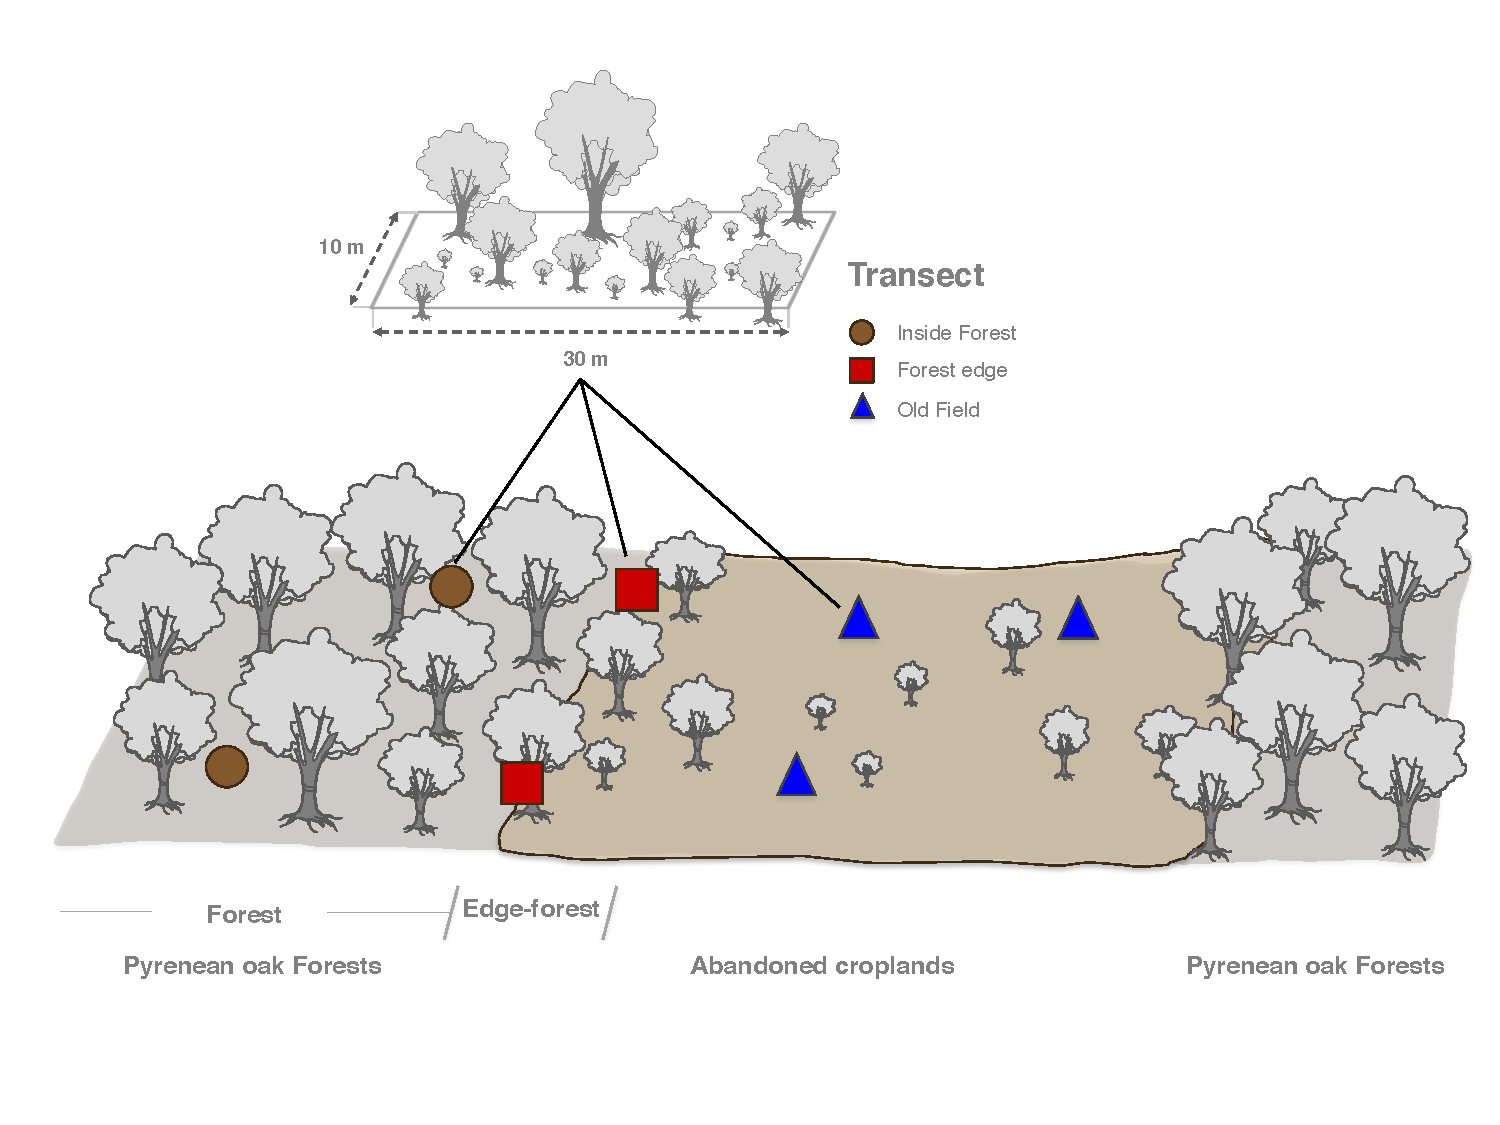
\includegraphics[width=\textwidth]{img/coloniza/coloniza-transectScheme.pdf}
    \caption{Sampling design. Vegetation transects were randomly placed in the old field (triangles), and inside the forest (circles) surrounding the old field. Several transects were also located at forest-old field edge (squares).}
    \label{fig:coloniza:transects}
\end{figure}

For each abandonment cropland, linear vegetation transects (30 m x 10 m) were randomly distributed in the old field; at the forest edges; and inside the surrounding forests (\figref{fig:coloniza:transects}). The numbers of transect within the old fields and surrounding forests were proportional to abandonment cropland size (Table 1). A total of 83 vegetation transects were sampled in autumn 2012.

In each vegetation transect all tree species were recorded, and tree height and diameter were measured. For each transect we computed the juvenile abundance as the number of individuals lower than 150 cm tall. We did not separate the generative and vegetative origins of young oaks, since it is difficult due to resprouting trait of this species. In addition to the juvenile abundance, we explored differences between several recruitment stages based on individual size \autocites[\emph{e.g}][]{Plieningeretal2010LargeScalePatterns}. We considered five size categories based in height (every 30 cm). All data were properly documented and published in an international repository \autocites[see][for a detailed description of the dataset]{PerezLuqueetal2015DatasetMIGRAME}. 

\subsection{Bird disperser}\label{sec:coloniza:bird}
To explore the main bird disperser in our study sites, we used bird censuses carried out by the Sierra Nevada Global Change Observatory. This dataset contains bird censuses at different ecosystems types of Sierra Nevada since 2008 \autocites[for more details see][]{BareaAzconetal2012PasseriformesOtrasa, PerezLuqueetal2016DatasetPasserine}. We only used data for the Eurasian jay (\emph{Garrulus glandarius}), since it is the main disperser of \Qpy \autocites{Gomez2003ImpactVertebrate}. As we are interested in the comparison of the Eurasian jay community between the two study sites, we computed the annual bird abundances (in terms of birds/10 ha) for each site during a 7-year period (2008-2013).  

The sampling procedures was the line-transect method with a bandwith of 50 m (25 m on each side). Transects length were 2.80 km for Cáñar site (CA), and 3.22 km for San Juan site (SJ). Sight and sound records within the sample area were accepted as contacts. All transects were sampled in the early morning, under appropriate climatic conditions. Eurasian jay abundance was calculated in terms of birds/10 ha. All counts in one month were averaged, and the yearly result was obtained from the average of all the months studied. For more details about bird censuses see \citet{BareaAzconetal2012PasseriformesOtrasa} and \citet{ZamoraBareaAzcon2015LongTermChanges}.

\subsection{Data analysis}\label{sec:coloniza:analysis}
We used the vegetation transects carried out inside the forest (habitat type = FOREST) to analyze the structure of the seed source (mature forest). Several parameters related to forests' structure and functioning were computed: tree density, juvenile abundance, tree species composition, tree size related statistics (\emph{i.e.} mean, median, maximum, 75 and 90 percentiles of tree-height), and basal area (BA). Differences between sites were assessed using the non-parametric Mann–Whitney U-test, since data does not met normality and/or homocedasticity assumptions. We also compared whether there was variation within transects belong to the same locality. ANOVA analysis were performed to explore differences of Bird disperser abundance (\emph{G. glandarius}) between sites and across years. 

The variation of the juvenile abundance between study sites, habitat type, and their interaction (site-habitat type), was analyzed using Generalized Linear Models with a Tweedie distribution with a log link (cita libro). Study sites and habitat type were the explanatory variables. Prior to the analysis, data exploration was applied following protocols described by \citet{Zuuretal2010ProtocolData} and \citet{IenoZuur2015BeginnerGuide}. As the dataset comprised count data, we initially used the Poisson and the Negative Binomial distribution. However, these models were overdispersed. A variance power parameter of 1.28 (1.20-1.40, 95\% confidence interval) were used in the Tweedie GLM model. This parameter was estimated using the \texttt{tweedie.profile} function of the \texttt{tweedie} R package \autocites{DunnSmyth2005SeriesEvaluation,Dunn2017Tweedie}. Model comparison (univariate models) were carried out using the Akaike's information criterion (AIC) \autocites{BurnhamAnderson2010ModelSelection}. The model accuracy was tested by Nagelkerke's pseudo-$R^2$, used as a measure of goodness of fit. The significance of the explanatory variables in the selected model was tested using the likelihood ratio tests (LRT). Wald z-tests and Tukey's HSD-corrected \emph{post hoc} comparisons were used to test for differences in juvenile abundance among sites and habitat-type. 

\begin{table}
\caption{Forest attributes of northern (SJ) and southern (CA) sites. U Mann-Withney statistics with significance at 0.05 level. Mean and SE are shown}
\centering
\resizebox{\linewidth}{!}{
\begin{tabular}[t]{ccccc}
\toprule
Variable & Southern site (CA) & Northern site (SJ) & U statistic & p value\\
\midrule
\% of Q. pyrenaica & 96.11 ± 1.28 & 100 ± 0 & 3.688 & 0.0001\\
Tree density (ind/ha) & 1671.11 ± 229.21 & 1587.5 ± 161.67 & 4.808 & 0.9369\\
Juvenile abundance (ind/ha) & 1004.44 ± 195.72 & 883.33 ± 127.18 & 4.852 & 0.7667\\
Adult abundance (ind/ha) & 584.44 ± 80.47 & 704.17 ± 63.31 & 4.448 & 0.1780\\
Maximum tree height (m) & 13.93 ± 0.65 & 13.75 ± 0.71 & 4.824 & 0.8736\\
Tree height mean (m) & 4.32 ± 0.6 & 5.09 ± 0.37 & 4.330 & 0.0855\\
Tree height median (m) & 3.19 ± 0.83 & 3.57 ± 0.66 & 4.564 & 0.3527\\
Tree height 75 percentile (m) & 5.73 ± 1.02 & 8.29 ± 0.6 & 4.343 & 0.0922\\
Tree height 90 percentile (m) & 10.07 ± 0.95 & 11.22 ± 0.54 & 4.605 & 0.4399\\
Basal Area (m2/ha) & 37.56 ± 4.23 & 33.58 ± 3.6 & 4.912 & 0.5400\\
\bottomrule
\end{tabular}}
\label{tab:coloniza:forest}
\end{table}

\begin{table}[]
\caption{Model selection for the oak juvenile abundance, sorted by minimum AICc value.}
\resizebox{\textwidth}{!}{%
\begin{tabular}{@{}llllll@{}}
\toprule
\textbf{model.name} & \textbf{df} & \textbf{logLik} & \textbf{AICc} & \Delta \textbf{AICc} & \textbf{Nagelkerke R\textsuperscript{2}} \\ \midrule
Habitat type + Site + Habitat type $\times$ Site & 6 & -221.89 & 457.78 & 0 & 0.970 \\
Habitat type + Site & 4 & -231.83 & 473.65 & 15.87 & 0.955 \\
Habitat type & 3 & -236.21 & 480.42 & 22.64 & 0.946 \\
Site & 2 & -291.06 & 588.12 & 130.34 & 0.116 \\
null model & 1 & -293.09 & 590.19 & 132.41 & 0 \\ \bottomrule
\end{tabular}%
}
\label{tab:coloniza:modelselection}
\end{table}

\section{Results}\label{sec:coloniza:results}

The forest structure of \Qpy woodlands did not show significant differences for the forest attributes between study sites  (\tabref{tab:coloniza:forest}). \Qpy woodlands of southern site (CA) showed higher tree density but smallest tree heights (mean, median and percentiles) than northern site (SJ) (\tabref{tab:coloniza:forest}). In addition, higher contribution of juvenile abundance was found for CA site, with also showed greater basal area than SJ site (\tabref{tab:coloniza:forest}).


In relation to the abundance of \emph{Garrulus glandarius}, no differences between study sites were found (\(F_{1,82}\)=2.387; p = 0.126; CA=1.69±0.21 and SJ = 1.33±0.22 birds/10ha), neither across years in the studied period (2008-2014) (\(F_{6,82}\)=1.234; p = 0.297). The interaction term was also no significant (\(F_{6,82}\)=1.26; p = 0.284).

The juvenile oak abundance model including all terms (\emph{i.e.} full model) showed higher strength of empirical support than did models for each of the independent variables (\emph{i.e.} univariate models) (\tabref{tab:coloniza:modelselection}). Oak juvenile abundance differ among habitat types (\(F_{2,77}\)=72.95; p < 0.0001), and between study sites (\(F_{1,77}\)=8.16; p = 0.0054; \tabref{tab:coloniza:anova}). 



\begin{figure}
    \centering
    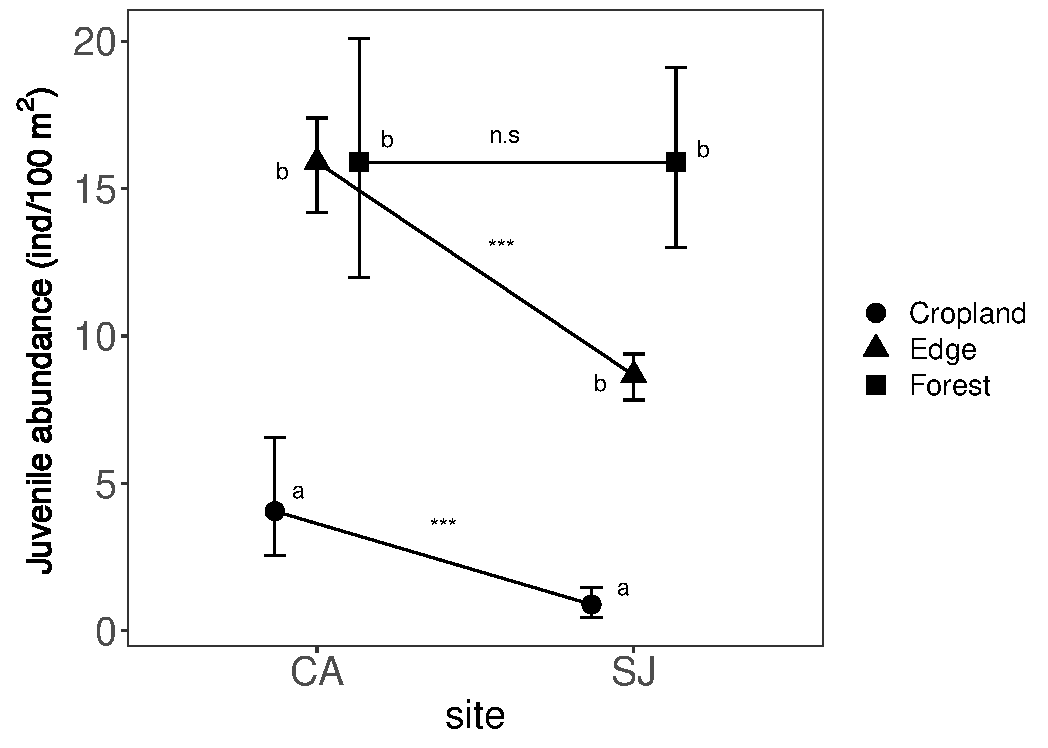
\includegraphics[width=\textwidth]{img/coloniza/coloniza-juvenile-interaction.pdf}
    \caption{Interaction plot for the oak juvenile abundance. Habitat-type differences within each site were indicated with different letters. Differences between sites for each habitat-type were indicated with asterisk.}
    \label{fig:coloniza:interaction}
\end{figure}

A decreasing gradient of oak-juvenile abundance was found across habitat-type, from higher values in forest type (15.90 ± 1.30 \juv) to lower values inside the old croplands (2.43 ± 0.55 \juv; \figref{fig:coloniza:interaction}). The abundance of oak juveniles in the old croplands of the southern site (CA) was significantly higher (4.06 ± 0.98 \juv) than in those of the northern site (SJ; 0.90 ± 0.26 \juv). 

The size distribution of juveniles was also different among the study sites (\figref{fig:coloniza:treeCategory}). An even size-distribution of oak juveniles was observed in the old croplands of northern site. Conversely, higher contribution of small oak juveniles (< 30 cm) were found at old croplands of southern site (\figref{fig:coloniza:treeCategory}). 

\begin{figure}
    \centering
    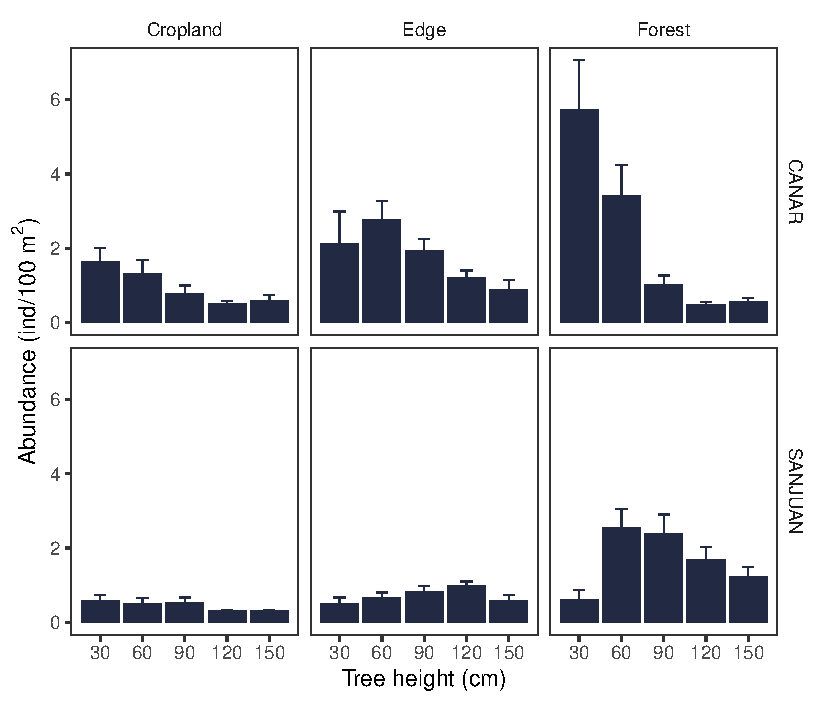
\includegraphics[width=\textwidth]{img/coloniza/coloniza-TreeCategory.pdf}
    \caption{Juvenile abundance classified by tree-size (see material and methods) by habitat-type in the two study sites. Mean and standard error are shown.}
    \label{fig:coloniza:treeCategory}
\end{figure}


A positive relation were found between the oak juvenile abundance and the estimate age of crop abandonment (\figref{fig:coloniza:ageCrop}) with higher oak juvenile abundances in the earlier abandonded croplands 

\section{Discussion}\label{sec:coloniza:disussion}


\begin{table}
\caption{ANOVA table of the selected GLM model for the abundance of \Qpy juvenile across study sites and habitat types. F-value and p-values are displayed.}
\centering
\begin{tabular}{lllll} 
\toprule
\textbf{Variable}        & \textbf{SS} & \textbf{df} & \textbf{F} & \textbf{p-value}  \\ 
\midrule
Habitat type             & 233.89      & 2           & 72.95      &  0.0001           \\
Site                     & 13.09       & 1           & 8.16       & 0.0054            \\
Habitat type $\times$ Site & 27.19       & 2           & 8.48       & 0.0004            \\
Residuals                & 123.43      & 77          &            &                   \\
\bottomrule
\end{tabular}
\label{tab:coloniza:anova}
\end{table}

\begin{figure}
    \centering
    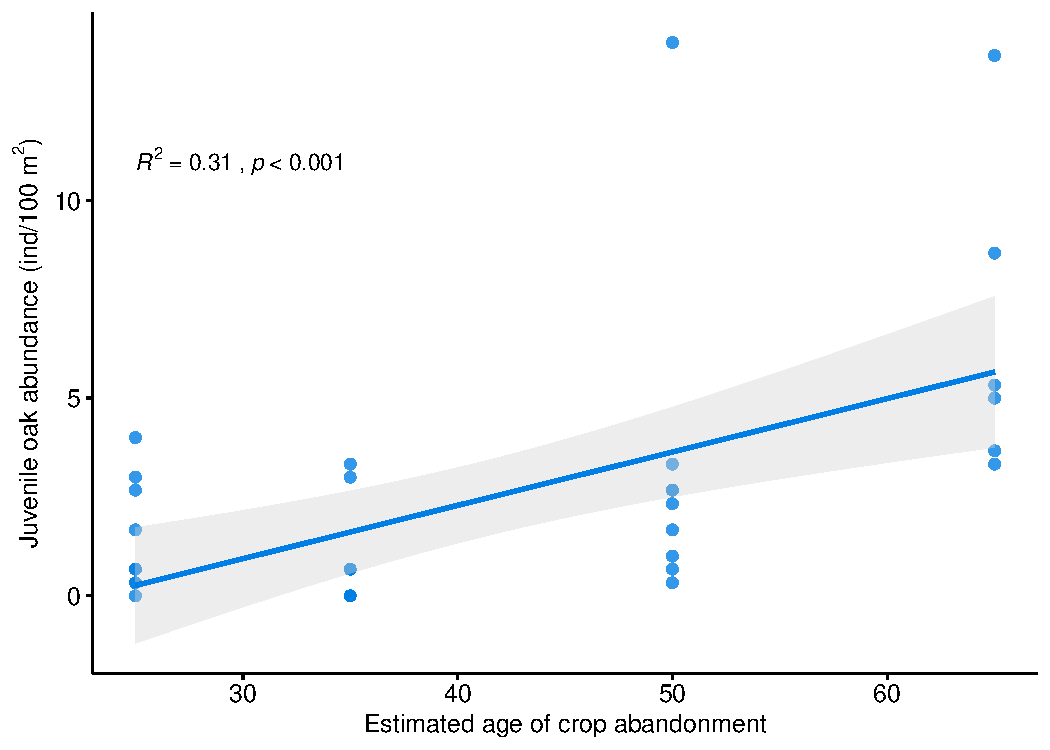
\includegraphics[width=\textwidth]{img/coloniza/coloniza-ageCrop.pdf}
    \caption{Relation of the juvenile oak abundance with the estimated age of crop abandonment.}
    \label{fig:coloniza:ageCrop}
\end{figure}



Agricultural practices were abandoned between 30-40 years ago in the study sites. Traditional grazing activities were detected in both sites, with more intensity in northern population (San Juan)


Notas de Puerta Piñero 2012 

On the other hand,
large-seed and biotic-dispersed species (e.g. Quercus sp) will be
short-distance passively dispersed and will require some degree
of previous perches and vegetation shelter to ensure effective biotic dispersal and further establishment (Gómez et al., 2008;
Gómez-Aparicio et al., 2009; García et al., 2010; Zamora et al.,
2010), which implies a slower colonization rate in open areas (such
as crops recently abandoned). 


 Although oaks are more abundant
than pines in the study area, oaks seem to colonize new areas at
a slower speed, owing to the need of secondary dispersers such
as Eurasian jay (Garrulus glandarius) or several species of mice
(mainly Apodemus sylvaticus and Mus spretus). The same pattern
is likely to appear in other biotic plant-frugivorous interactions
requiring some degree of forest structure and/or shelter to attain
effective seed dispersal (Castro et al., 2010; Gómez-Aparicio et al., 2009; Rost et al., 2009; Lehouck et al., 2009; Uriarte et al., 2011). Indeed, dispersal limitation has been proposed as more critical than recruitment limitation for the colonization of old-forestspecialized plant species after agriculture abandonment (reviewed in Hermy and Verheyen, 2007).


Our results suggest that the longer the time since crop abandonment, the more heterogeneity in species and diversity of functional responses to potential perturbations are present, as
previously reported (Rudel et al., 2005; Fraterrigo et al., 2006; Hermy and Verheyen, 2007),

On the whole, our findings highlight that predictions on how
extensive disturbances such as fire affect the regeneration and further distribution of plants, should take into account also historical
land trajectories. 



- Edad de abandono
Puerta-Piñero et al 2012
 Furthermore, the longer since crop abandonment translates into a faster post-fire recovery
 
 
 
--- 
Notas from Baraza et al. 2006 https://onlinelibrary.wiley.com/doi/abs/10.1111/j.0030-1299.2006.14265.x

Importancia del contexto en el efecto de la herbivoría

The community context in which interaction takes place, namely the characteristics of the neighbours and the intensity of herbivore pressure, are determining factors for understanding and predicting the damage undergone by a target plant species.





Hermy, M., Verheyen, K., 2007. Legacies of the past in the present-day forest
biodiversity: a review of past land-use effects on forest plant species
composition and diversity. Ecol. Res. 22, 361–371. http://dx.doi.org/10.1007/
s11284-007-0354-3.
ICONA, 1993–2000. Segund


Piusi (2000) reforestation depens on the inrecation of basic factors such us the availibility of propagules, the characteristic of disseminatiojn, the competition of the tre seedlings and. herbaceous bvege4tation and the former land use. Tambien se ha dicho que es importante la distancia a la fuente 